\documentclass[a4paper, 12pt]{article}		% general format

%%%% Charset
\usepackage{cmap}							% make PDF files searchable and copyable
\usepackage[utf8]{inputenc}					% accept different input encodings
\usepackage[T2A]{fontenc}					% russian font
\usepackage[russian]{babel}					% multilingual support (T2A)

%%%% Graphics
\usepackage[dvipsnames]{xcolor}			% driver-independent color extensions
\usepackage{graphicx}						% enhanced support for graphics
\usepackage{wrapfig}						% produces figures which text can flow around

%%%% Math
\usepackage{amsmath}						% American Mathematical Society (AMS) math facilities
\usepackage{amsfonts}						% fonts from the AMS
\usepackage{amssymb}						% additional math symbols

%%%% Typograpy (don't forget about cm-super)
\usepackage{microtype}						% subliminal refinements towards typographical perfection
\linespread{1.3}							% line spacing
\usepackage[left=2.5cm, right=1.5cm, top=2.5cm, bottom=2.5cm]{geometry}
\setlength{\parindent}{0pt}					% we don't want any paragraph indentation
%\renewcommand{\chaptername}{}

%%%% Other
\usepackage{url}							% verbatim with URL-sensitive line breaks
%\DeclareUnicodeCharacter{00A0}{~}

%------------------------------------------------------------------------------
\usepackage{listings}						% typeset source code listings

% Цвета для кода
\definecolor{string}{HTML}{101AF9}			% цвет строк в коде
\definecolor{comment}{HTML}{0C2612}		% цвет комментариев в коде
\definecolor{keyword}{HTML}{5F1441}		% цвет ключевых слов в коде
\definecolor{morecomment}{HTML}{8000FF}	% цвет include и других элементов в коде
\definecolor{captiontext}{HTML}{FFFFFF}	% цвет текста заголовка в коде
\definecolor{captionbk}{HTML}{999999}		% цвет фона заголовка в коде
\definecolor{bk}{HTML}{FFFFFF}				% цвет фона в коде
\definecolor{frame}{HTML}{999999}			% цвет рамки в коде

% Настройки отображения кода
\lstset{
	language=C++,							% Язык кода по умолчанию
	morekeywords={*,...},					% если хотите добавить ключевые слова, то добавляйте
	% Цвета
	keywordstyle=\color{keyword}\ttfamily\bfseries,
	stringstyle=\color{string}\ttfamily,
	commentstyle=\color{comment}\ttfamily\itshape,
	morecomment=[l][\color{morecomment}]{\#},
	% Настройки отображения
	breaklines=true,						% Перенос длинных строк
	basicstyle=\ttfamily\footnotesize,		% Шрифт для отображения кода
	backgroundcolor=\color{bk},				% Цвет фона кода
	%frame=lrb,xleftmargin=\fboxsep,xrightmargin=-\fboxsep, % Рамка, подогнанная к заголовку
	frame=tblr								% draw a frame at all sides of the code block
	rulecolor=\color{frame},				% Цвет рамки
	tabsize=2,								% tab space width
	showstringspaces=false,					% don't mark spaces in strings
	% Настройка отображения номеров строк. Если не нужно, то удалите весь блок
	numbers=left,							% Слева отображаются номера строк
	stepnumber=1,							% Каждую строку нумеровать
	numbersep=5pt,							% Отступ от кода
	numberstyle=\small\color{black},		% Стиль написания номеров строк
	% Для отображения русского языка
	extendedchars=true,
	literate={Ö}{{\"O}}1
	 	{Ä}{{\"A}}1
	 	{Ü}{{\"U}}1
		{ß}{{\ss}}1
		{ü}{{\"u}}1
		{ä}{{\"a}}1
		{ö}{{\"o}}1
		{~}{{\textasciitilde}}1
		{а}{{\selectfont\char224}}1
		{б}{{\selectfont\char225}}1
		{в}{{\selectfont\char226}}1
		{г}{{\selectfont\char227}}1
		{д}{{\selectfont\char228}}1
		{е}{{\selectfont\char229}}1
		{ё}{{\"e}}1
		{ж}{{\selectfont\char230}}1
		{з}{{\selectfont\char231}}1
		{и}{{\selectfont\char232}}1
		{й}{{\selectfont\char233}}1
		{к}{{\selectfont\char234}}1
		{л}{{\selectfont\char235}}1
		{м}{{\selectfont\char236}}1
		{н}{{\selectfont\char237}}1
		{о}{{\selectfont\char238}}1
		{п}{{\selectfont\char239}}1
		{р}{{\selectfont\char240}}1
		{с}{{\selectfont\char241}}1
		{т}{{\selectfont\char242}}1
		{у}{{\selectfont\char243}}1
		{ф}{{\selectfont\char244}}1
		{х}{{\selectfont\char245}}1
		{ц}{{\selectfont\char246}}1
		{ч}{{\selectfont\char247}}1
		{ш}{{\selectfont\char248}}1
		{щ}{{\selectfont\char249}}1
		{ъ}{{\selectfont\char250}}1
		{ы}{{\selectfont\char251}}1
		{ь}{{\selectfont\char252}}1
		{э}{{\selectfont\char253}}1
		{ю}{{\selectfont\char254}}1
		{я}{{\selectfont\char255}}1
		{А}{{\selectfont\char192}}1
		{Б}{{\selectfont\char193}}1
		{В}{{\selectfont\char194}}1
		{Г}{{\selectfont\char195}}1
		{Д}{{\selectfont\char196}}1
		{Е}{{\selectfont\char197}}1
		{Ё}{{\"E}}1
		{Ж}{{\selectfont\char198}}1
		{З}{{\selectfont\char199}}1
		{И}{{\selectfont\char200}}1
		{Й}{{\selectfont\char201}}1
		{К}{{\selectfont\char202}}1
		{Л}{{\selectfont\char203}}1
		{М}{{\selectfont\char204}}1
		{Н}{{\selectfont\char205}}1
		{О}{{\selectfont\char206}}1
		{П}{{\selectfont\char207}}1
		{Р}{{\selectfont\char208}}1
		{С}{{\selectfont\char209}}1
		{Т}{{\selectfont\char210}}1
		{У}{{\selectfont\char211}}1
		{Ф}{{\selectfont\char212}}1
		{Х}{{\selectfont\char213}}1
		{Ц}{{\selectfont\char214}}1
		{Ч}{{\selectfont\char215}}1
		{Ш}{{\selectfont\char216}}1
		{Щ}{{\selectfont\char217}}1
		{Ъ}{{\selectfont\char218}}1
		{Ы}{{\selectfont\char219}}1
		{Ь}{{\selectfont\char220}}1
		{Э}{{\selectfont\char221}}1
		{Ю}{{\selectfont\char222}}1
		{Я}{{\selectfont\char223}}1
		{і}{{\selectfont\char105}}1
		{ї}{{\selectfont\char168}}1
		{є}{{\selectfont\char185}}1
		{ґ}{{\selectfont\char160}}1
		{І}{{\selectfont\char73}}1
		{Ї}{{\selectfont\char136}}1
		{Є}{{\selectfont\char153}}1
		{Ґ}{{\selectfont\char128}}1
}

% Для настройки заголовка кода
\usepackage{caption}
\DeclareCaptionFont{white}{\color{сaptiontext}}
\DeclareCaptionFormat{listing}{\parbox{\linewidth}{\colorbox{сaptionbk}{\parbox{\linewidth}{#1#2#3}}\vskip-4pt}}
%\captionsetup[lstlisting]{format=listing,labelfont=white,textfont=white}
\renewcommand{\lstlistingname}{Листинг} % Переименование Listings в нужное именование структуры

%------------------------------------------------------------------------------
\begin{document}

\begin{titlepage}
\thispagestyle{empty}

\begin{center}
Санкт-Петербургский государственный политехнический университет \\
Институт Информационных Технологий и Управления \\*
Кафедра компьютерных систем и программных технологий \\*
\hrulefill
\end{center}

\vspace{18em}

\begin{center}
\Large Отчёт по расчётной работе № 3 \\ по предмету «Системное программное обеспечение» \\
\end{center}

\vspace{1em}

% \linebreak
\begin{center}
\textsc{\textbf{Примитивы синхронизации в ОС Windows}}
\end{center}

\vspace{16em}

\begin{flushleft}
Работу выполнил студент гр. 53501/3\hrulefill Мартынов С. А. \\
\vspace{1.5em}
Работу принял преподаватель \hrulefill Душутина Е. В. \\
\end{flushleft}

\vspace{\fill}

\begin{center}
Санкт-Петербург \\
2014
\end{center}

\end{titlepage}
%------------------------------------------------
\setcounter{page}{2}
\tableofcontents
%------------------------------------------------
\newpage
\section*{Постановка задачи}
\addcontentsline{toc}{section}{Постановка задачи}

В рамках данной работы необходимо ознакомиться с основными примитивами синхронизации в ОС Windows, и выполнить следующие задачи:
\vspace{3em}

Потоки разделяют целочисленный массив, в который заносятся производимые и извлекаются потребляемые данные. Для наглядности и контроля за происходящим в буфер помещается наращиваемое значение, однозначно идентифицирующее производителя и номер его очередной посылки.

Код должен удовлетворять трем требованиям:
\begin{itemize}
\item потребитель не должен пытаться извлечь значение из буфера, если буфер пуст;
\item производитель не должен пытаться поместить значение в буфер, если буфер полон;
\item состояние буфера должно описываться общими переменными (индексами, счётчиками, указателями связанных списков и т.д.).
\end{itemize}

Задание необходимо выполнить различными способами, применив следующие средства синхронизации доступа к разделяемому ресурсу:
\begin{itemize}
\item Мьютексы;
\item Семафоры;
\item Критические секции;
\item Объекты события;
\item Условные переменные;
\item Функции ожидания.
\end{itemize}

Создать аналогичные программы для множества потоков, количество которых можно задать из командной строки.

Программы должны предоставлять возможность завершения по таймеру либо по команде оператора.
\vspace{3em}

Отчёт должен содержать:
\begin{enumerate}
\item Результаты выполнения предложенных в методическоом пособии программ и их анализ.
\item Рещение задачи читатели-писатели таким образом, чтобы читатели не имели доступа к памяти по записи.
\item Более рациональное решение задачи читатели-писатель, используя другие средства синхронизации или их сочетание. Объяснить и подтвердить экспериментально улучшение характеристик взаимодействия.
\item Клиент-серверное приложение для полной задачи читатели-писатели с собственной системой ограничений на доступ каждого читателя к информации.
\item Программу читатели-писатели для сетевого функционирования (для этого необходимо выбрать подходящие средства IPC и синхронизации).
\item Решение задачи производители-потребители (разница с предыдущей задачей в возможности модификации считываемых данных).
\item Задачу "обедающие философы" с обоснованием выбранных средств синхронизации.
\end{enumerate}

\newpage
%------------------------------------------------
\section*{Введение}
\addcontentsline{toc}{section}{Введение}

Исходный код всех представленных листингов доступен по адресу \\ \url{https://github.com/SemenMartynov/SPbPU_SystemProgramming}.

\newpage
%------------------------------------------------
\section{Примитивы синхронизации}

Код задач в данном разделе разбит на файлы. Некоторые файлы (такие как система логирования) в разных проектах содержат одинаковый код. Для простоты восприятия информации, они вынесены в этот раздел (полную версию исходных кодов можно получит по ссылке на гитхаб, приведённой во введении).

\lstinputlisting[language=C++, caption={Реализация класса логера}]
{../../SynchronizationPrimitives/Mutex/Logger.cpp}

\lstinputlisting[language=C++, caption={Сервисные функции}]
{../../SynchronizationPrimitives/Mutex/utils.cpp}

\newpage
%------------------------------------------------
\subsection{Использование мьютексов}

\begin{figure}[h!]
\centering
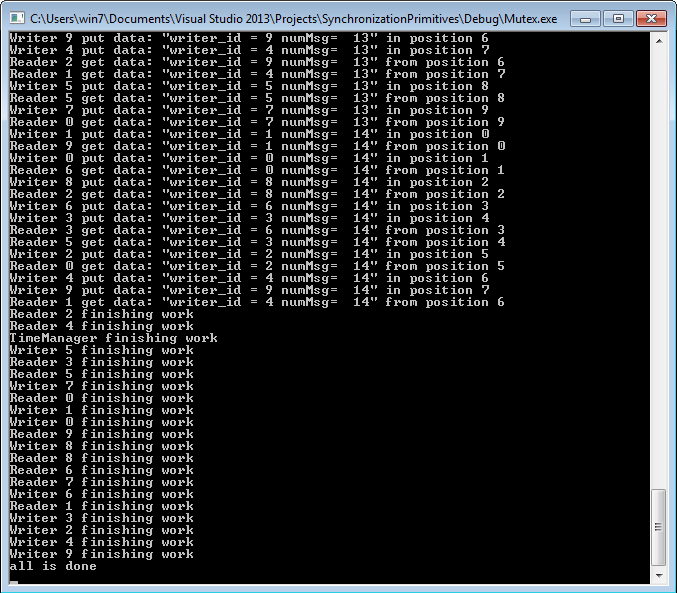
\includegraphics[scale=1]{res/001}
\caption{Использование мьютексов.}
\end{figure}

\lstinputlisting[language=C++, caption={Основной файл}]
{../../SynchronizationPrimitives/Mutex/main.cpp}

\lstinputlisting[language=C++, caption={Потоки писатели}]
{../../SynchronizationPrimitives/Mutex/threadWriter.cpp}

\lstinputlisting[language=C++, caption={Потоки читатели}]
{../../SynchronizationPrimitives/Mutex/threadReader.cpp}


\newpage
%------------------------------------------------
\subsection{Использование семафоров}

\begin{figure}[h!]
\centering
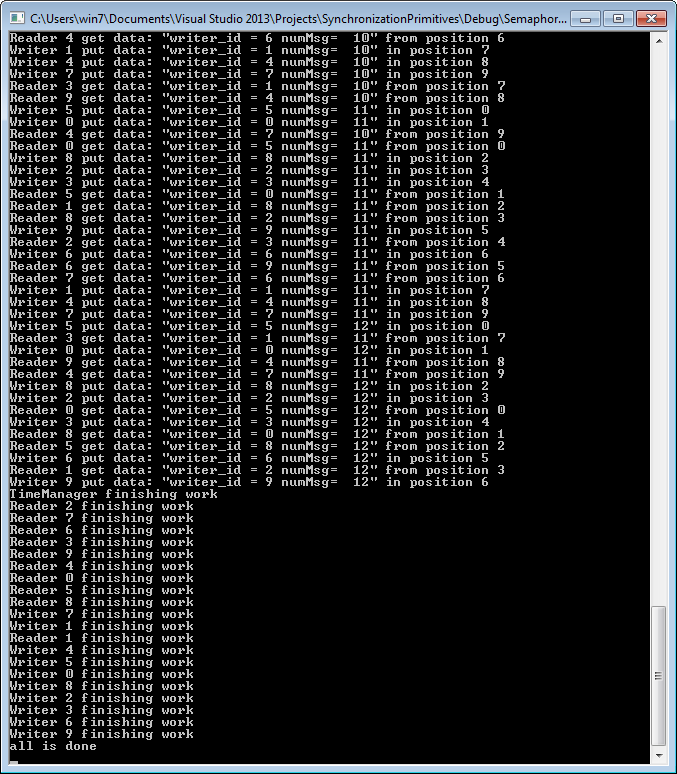
\includegraphics[scale=1]{res/002}
\caption{Использование семафоров.}
\end{figure}

\lstinputlisting[language=C++, caption={Основной файл}]
{../../SynchronizationPrimitives/Semaphore/main.cpp}

\lstinputlisting[language=C++, caption={Потоки писатели}]
{../../SynchronizationPrimitives/Semaphore/threadWriter.cpp}

\lstinputlisting[language=C++, caption={Потоки читатели}]
{../../SynchronizationPrimitives/Semaphore/threadReader.cpp}

\newpage
%------------------------------------------------
\subsection{Критические секции}

\begin{figure}[h!]
\centering
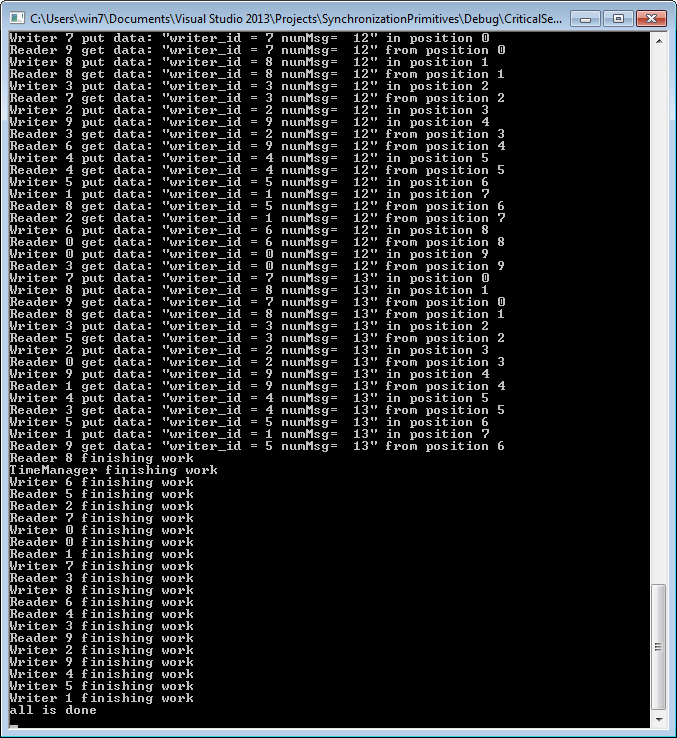
\includegraphics[scale=1]{res/003}
\caption{Критические секции.}
\end{figure}

\lstinputlisting[language=C++, caption={Основной файл}]
{../../SynchronizationPrimitives/CriticalSection/main.cpp}

\lstinputlisting[language=C++, caption={Потоки писатели}]
{../../SynchronizationPrimitives/CriticalSection/threadWriter.cpp}

\lstinputlisting[language=C++, caption={Потоки читатели}]
{../../SynchronizationPrimitives/CriticalSection/threadReader.cpp}

\newpage
%------------------------------------------------
\subsection{Объекты-события в качестве средства синхронизации}

\begin{figure}[h!]
\centering
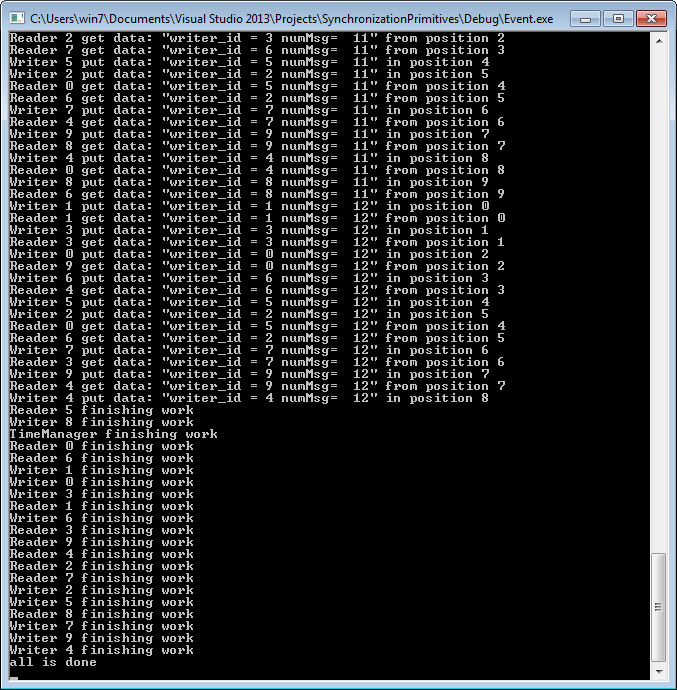
\includegraphics[scale=1]{res/004}
\caption{Объекты-события в качестве средства синхронизации.}
\end{figure}

\lstinputlisting[language=C++, caption={Основной файл}]
{../../SynchronizationPrimitives/Event/main.cpp}

\lstinputlisting[language=C++, caption={Потоки писатели}]
{../../SynchronizationPrimitives/Event/threadWriter.cpp}

\lstinputlisting[language=C++, caption={Потоки читатели}]
{../../SynchronizationPrimitives/Event/threadReader.cpp}

\newpage
%------------------------------------------------
\subsection{Условные переменные}

\begin{figure}[h!]
\centering
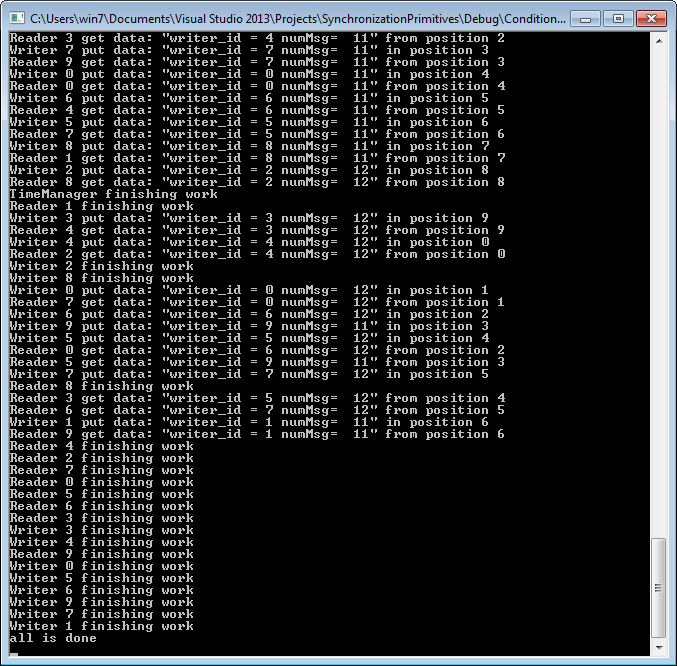
\includegraphics[scale=1]{res/005}
\caption{Условные переменные.}
\end{figure}

\lstinputlisting[language=C++, caption={Основной файл}]
{../../SynchronizationPrimitives/ConditionVariable/main.cpp}

\lstinputlisting[language=C++, caption={Потоки писатели}]
{../../SynchronizationPrimitives/ConditionVariable/threadWriter.cpp}

\lstinputlisting[language=C++, caption={Потоки читатели}]
{../../SynchronizationPrimitives/ConditionVariable/threadReader.cpp}

\newpage
%------------------------------------------------
\subsection{Задача читатели-писатели (для потоков одного процесса)}

Рассмотрим частный случай этой задачи для демонстрации использования объектов-событий для синхронизации доступа к памяти.


Задание: необходимо решить задачу одного писателя и N читателей. Для синхронизации разрешено использовать только объекты-события, в качестве разделяемого ресурса -- разделяемую память (share memory). Писатель пишет в share memory сообщение и ждет, пока все читатели не прочитают данное сообщение.


Задача должна быть решена сначала для потоков, принадлежащих одному процессу, а затем – разным независимым процессам.

\begin{figure}[h!]
\centering
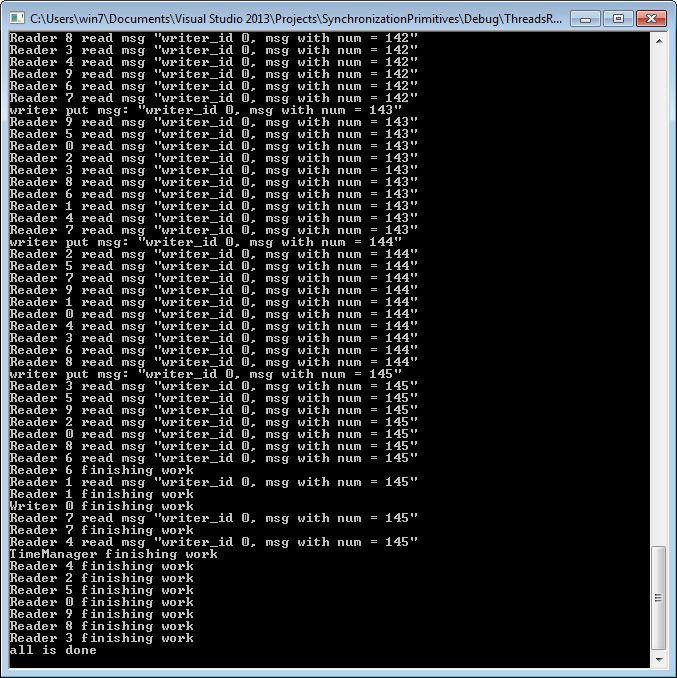
\includegraphics[scale=1]{res/006}
\caption{Задача читатели и писатели.}
\end{figure}

\lstinputlisting[language=C++, caption={Основной файл}]
{../../SynchronizationPrimitives/ThreadsReaderWriter/main.cpp}

\lstinputlisting[language=C++, caption={Потоки писатели}]
{../../SynchronizationPrimitives/ThreadsReaderWriter/threadWriter.cpp}

\lstinputlisting[language=C++, caption={Потоки читатели}]
{../../SynchronizationPrimitives/ThreadsReaderWriter/threadReader.cpp}

\newpage
%------------------------------------------------
\subsection{Задача читатели-писатели (для потоков разных процессов)}

В данной программе главный поток и поток-писатель будут принадлежать одному процессу, потоки-читатели – разным. Главный процесс создает процессы-читатели и 2 потока: писатель и планировщик. Для наглядности каждый процесс-читатель связан со своей консолью.

\begin{figure}[h!]
\centering
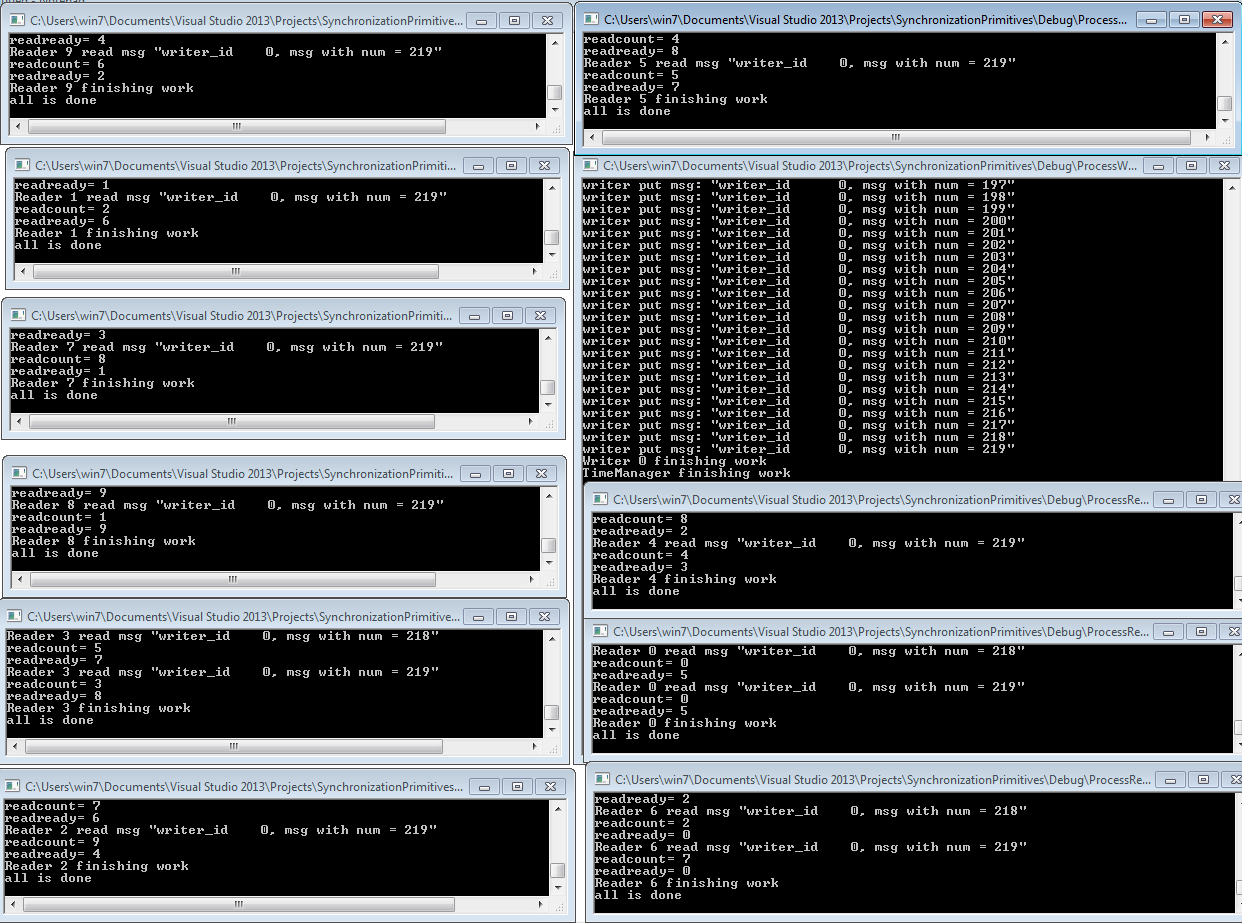
\includegraphics[scale=0.50]{res/007}
\caption{Решение задачи читатели-писатели для потоков.}
\end{figure}

\lstinputlisting[language=C++, caption={Основной файл}]
{../../SynchronizationPrimitives/ProcessWriter/main.cpp}

\lstinputlisting[language=C++, caption={Потоки писатели}]
{../../SynchronizationPrimitives/ProcessWriter/threadWriter.cpp}

\lstinputlisting[language=C++, caption={Запуск кллиентских процессов}, firstline=20, lastline=76]
{../../SynchronizationPrimitives/ProcessWriter/utils.cpp}

\lstinputlisting[language=C++, caption={Потоки читатели}]
{../../SynchronizationPrimitives/ProcessReader/main.cpp}


\newpage
%------------------------------------------------
\section{Модификация задачи читатели-писатели}

Читатели не имеют доступа к памяти по записи.

\begin{figure}[h!]
\centering
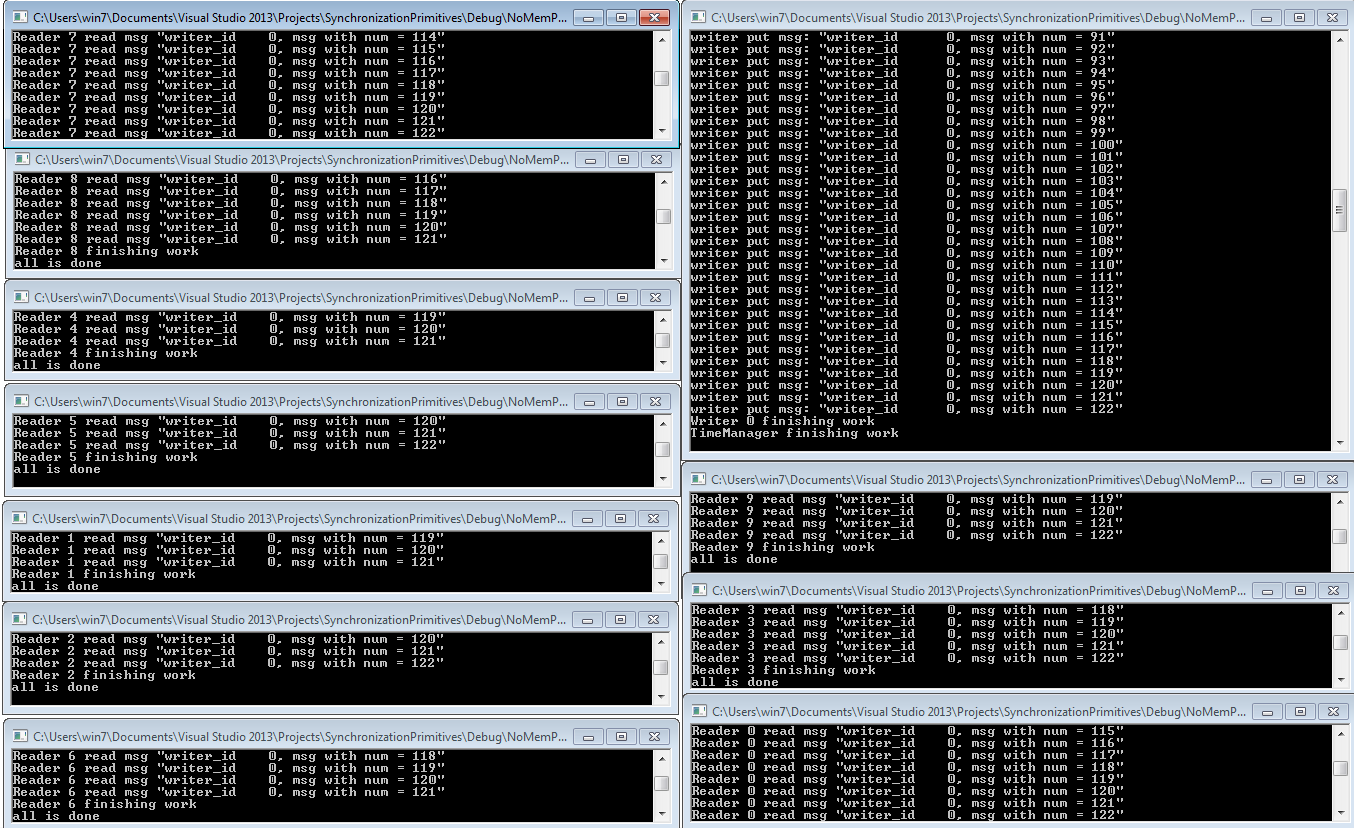
\includegraphics[scale=0.50]{res/008}
\caption{Модификация задачи читатели-писатели.}
\end{figure}

\lstinputlisting[language=C++, caption={Основной файл}]
{../../SynchronizationPrimitives/NoMemProcessWriter/main.cpp}

\lstinputlisting[language=C++, caption={Потоки писатели}]
{../../SynchronizationPrimitives/NoMemProcessWriter/threadWriter.cpp}

\lstinputlisting[language=C++, caption={Запуск кллиентских процессов}, firstline=20, lastline=76]
{../../SynchronizationPrimitives/NoMemProcessWriter/utils.cpp}

\lstinputlisting[language=C++, caption={Потоки читатели}]
{../../SynchronizationPrimitives/NoMemProcessReader/main.cpp}

\newpage
%------------------------------------------------
\section*{Заключение}
\addcontentsline{toc}{section}{Заключение}


\end{document}
